\documentclass{article}
\usepackage{graphicx} % Required for inserting images
\usepackage{enumitem}
\usepackage{tikz}

\title{\vspace{-2.0cm}INF 273 - Assignment 1}
\author{Runar Fosse}
\date{}

\begin{document}

\maketitle

\begin{enumerate}[label=(\alph*)]
    \item The problem requires us to have one mothership, visiting at least one port (different from the continental port, which always is assumed start and end port). We can also use however many daughterships we want, visiting other ports in a subtour (starting and ending at the port they disembarked from the mothership).
    \\[10pt]
    A good solution representation is one which encompasses all feasible solutions to the problem, while still not being so large that it covers a lot of invalid solutions. One should try to prevent duplicate solutions from being stored as different representations, and a solution representation should be easy to modify.
    \\[10pt]
    We can store the route of the mothership as a list of node values. Whenever we want to drop off daughterships, we can insert a negative integer in the list. The absolute value of this integer denotes the "id" of said daughtership which is dropped off. Storing the integer as a negative means we easily can identify whenever we drop off any daughterships. For each daughtership we can store a seperate list containing their route in the same way we represented the mothership's route (just without any negative numbers).
    \\[10pt]
    The daughterships do not need to store the port they start or end at, as this will be equal to the port where the mothership was located when they disembarked. We know implicitly given the requirements that at the start of a given daughtership's route they are located at this current port, and they will return to this same port at the end of their list.
    \\[10pt]
    For the solution to the problem given in the lecture slides (\#1-a), my suggestion of a good solution representation would look something like this:
    \\[30pt]
    
    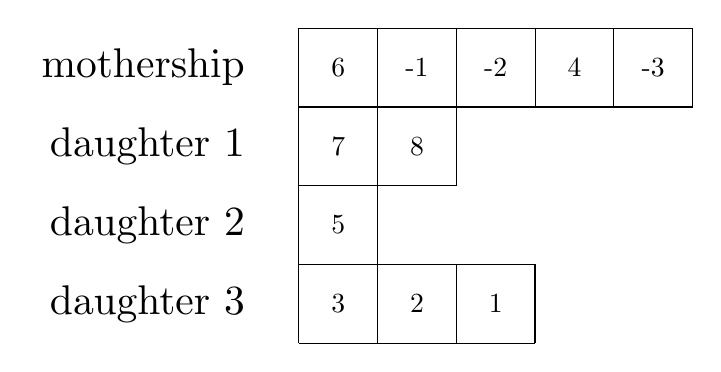
\begin{tikzpicture}
        \draw (0, 3) grid (5, 4);
        \node[scale=1.5,anchor=east] at (-0.5, 3.5) {mothership};
        \node[scale=1] at (0.5, 3.5) {6};
        \node[scale=1] at (1.5, 3.5) {-1};
        \node[scale=1] at (2.5, 3.5) {-2};
        \node[scale=1] at (3.5, 3.5) {4};
        \node[scale=1] at (4.5, 3.5) {-3};

        \draw (0, 2) grid (2, 3);
        \node[scale=1.5,anchor=east] at (-0.5, 2.5) {daughter 1};
        \node[scale=1] at (0.5, 2.5) {7};
        \node[scale=1] at (1.5, 2.5) {8};

        \draw (0, 1) grid (1, 2);
        \node[scale=1.5,anchor=east] at (-0.5, 1.5) {daughter 2};
        \node[scale=1] at (0.5, 1.5) {5};

        \draw (0, 0) grid (3, 1);
        \node[scale=1.5,anchor=east] at (-0.5, 0.5) {daughter 3};
        \node[scale=1] at (0.5, 0.5) {3};
        \node[scale=1] at (1.5, 0.5) {2};
        \node[scale=1] at (2.5, 0.5) {1};
    \end{tikzpicture}

    \item The problem requires us to deliver packages to all nodes given. We control a truck, which delivers packages in a tour starting and ending at node 0. The truck also has two drones which it can send out to deliver a single package at a time, before they have to return to the truck at a different node to retrieve another one.
    \\[10pt]
    We can represent the solution as a matrix. The first row denotes the route of the truck, containing the nodes it visits, and starting and ending with 0. Every node value is stored twice, one denoting arriving at a node while another one denoting departure (this is swapped for node 0, as the truck initially is located here).
    \\[10pt]
    The other two rows denote the route of the drones. As this is a matrix, these rows will have the same length as the truck's row. We can default the value of a given drone-row's index to 0, denoting it just idles (does nothing, e.g. is aboard the truck). Whenever the truck departures from a node in which it wants to send out a given drone, we can set the value of that drone's row at the current index to the "id" of the node it should deliver a package to. The truck then travels further along its path. As the drone can return to the truck at any given later node, we can set the value of the drone's row at that index in which it returns to the truck (this will be an index in which the truck arrives at a new node) to -1, denoting it returns to the truck.
    \\[10pt]
    By duplicating each node value (denoting when truck arrives and departures), it becomes really easy to represent when a drone leaves from the truck and when it returns. It will also be possible to have a drone return and leave again on the same node.
    \\[10pt]
    For the solution to the problem given in the lecture slides (\#1-b), my suggestion of a good solution representation would look something like this:
    \\[30pt]

    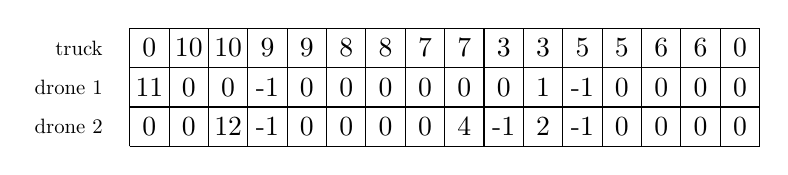
\begin{tikzpicture}
        \draw[scale=0.5] (0, 0) grid (16, 3);
        \node[scale=0.75,anchor=east] at (-0.5/2, 2.5/2) {truck};
        \node[scale=1] at (0.5/2, 2.5/2) {0};
        \node[scale=1] at (1.5/2, 2.5/2) {10};
        \node[scale=1] at (2.5/2, 2.5/2) {10};
        \node[scale=1] at (3.5/2, 2.5/2) {9};
        \node[scale=1] at (4.5/2, 2.5/2) {9};
        \node[scale=1] at (5.5/2, 2.5/2) {8};
        \node[scale=1] at (6.5/2, 2.5/2) {8};
        \node[scale=1] at (7.5/2, 2.5/2) {7};
        \node[scale=1] at (8.5/2, 2.5/2) {7};
        \node[scale=1] at (9.5/2, 2.5/2) {3};
        \node[scale=1] at (10.5/2, 2.5/2) {3};
        \node[scale=1] at (11.5/2, 2.5/2) {5};
        \node[scale=1] at (12.5/2, 2.5/2) {5};
        \node[scale=1] at (13.5/2, 2.5/2) {6};
        \node[scale=1] at (14.5/2, 2.5/2) {6};
        \node[scale=1] at (15.5/2, 2.5/2) {0};

        \node[scale=0.75,anchor=east] at (-0.5/2, 1.5/2) {drone 1};
        \node[scale=1] at (0.5/2, 1.5/2) {11};
        \node[scale=1] at (1.5/2, 1.5/2) {0};
        \node[scale=1] at (2.5/2, 1.5/2) {0};
        \node[scale=1] at (3.5/2, 1.5/2) {-1};
        \node[scale=1] at (4.5/2, 1.5/2) {0};
        \node[scale=1] at (5.5/2, 1.5/2) {0};
        \node[scale=1] at (6.5/2, 1.5/2) {0};
        \node[scale=1] at (7.5/2, 1.5/2) {0};
        \node[scale=1] at (8.5/2, 1.5/2) {0};
        \node[scale=1] at (9.5/2, 1.5/2) {0};
        \node[scale=1] at (10.5/2, 1.5/2) {1};
        \node[scale=1] at (11.5/2, 1.5/2) {-1};
        \node[scale=1] at (12.5/2, 1.5/2) {0};
        \node[scale=1] at (13.5/2, 1.5/2) {0};
        \node[scale=1] at (14.5/2, 1.5/2) {0};
        \node[scale=1] at (15.5/2, 1.5/2) {0};

        \node[scale=0.75,anchor=east] at (-0.5/2, 0.5/2) {drone 2};
        \node[scale=1] at (0.5/2, 0.5/2) {0};
        \node[scale=1] at (1.5/2, 0.5/2) {0};
        \node[scale=1] at (2.5/2, 0.5/2) {12};
        \node[scale=1] at (3.5/2, 0.5/2) {-1};
        \node[scale=1] at (4.5/2, 0.5/2) {0};
        \node[scale=1] at (5.5/2, 0.5/2) {0};
        \node[scale=1] at (6.5/2, 0.5/2) {0};
        \node[scale=1] at (7.5/2, 0.5/2) {0};
        \node[scale=1] at (8.5/2, 0.5/2) {4};
        \node[scale=1] at (9.5/2, 0.5/2) {-1};
        \node[scale=1] at (10.5/2, 0.5/2) {2};
        \node[scale=1] at (11.5/2, 0.5/2) {-1};
        \node[scale=1] at (12.5/2, 0.5/2) {0};
        \node[scale=1] at (13.5/2, 0.5/2) {0};
        \node[scale=1] at (14.5/2, 0.5/2) {0};
        \node[scale=1] at (15.5/2, 0.5/2) {0};
    \end{tikzpicture}
    
\end{enumerate}

\end{document}
